%!TEX root = ../../Paper.tex

\chapter{Trend Analysis on Twitter: Concept}
\label{cha:trend-detection-concept}

\section{Related Work}
\label{sec:related-work}
The analysis of microblogging data has been shown to provide new and not otherwise attainable information and it is, therefore, an important resource for big social data analysis. There are various tools to collect, analyze and visualize certain aspects of Twitter data. The MapD tweetmap\footnote{\url{http://mapd.csail.mit.edu/tweetmap-desktop} \accessednote} enables users to analyze nearly 350 million historical geolocated Tweets from January 2011 to September 2013 in milliseconds and visualize the results on a map. Sentiment Viz is a web application that allows to track certain keywords to analyze the sentiment of corresponding Tweets in real-time and visualize the results using different techniques \cite{healy2014twittersentiment}. The Arizona State University developed the TweetTracker and TweetXplorer tools to track, analyze, visualize and understand the activity on Twitter. TweetTracker is \enquote{capable of monitoring and analyzing location and keyword specific Tweets with near-real-time trending, data reduction, historical review, and integrated data mining tools} \cite[1]{kumar2011tweettracker}, whereas TweetXplorer provides a comprehensive set of effective visualization techniques \cite{morstatter2013understanding}. Furthermore, other tools are specialized in specific use cases such as the weather sentiment prediction application\footnote{\url{http://www.sproutloop.com/prediction_demo} \accessednote}, for analyzing the sentiment about the weather at a specific location, and trendsmap\footnote{\url{http://trendsmap.com} \accessednote}, for visualizing upcoming localized trends on a map. Furthermore, the company \textit{Dataminr} scans Twitter for relevant messages characterized by \enquote{the right combination of language, context and location} to detect \enquote{breaking- and money-making-news} \cite{alcorn2013stockmarket}.

Moreover, Naaman et al. used twitter to \enquote{identify important dimensions according to which trends can be categorized, as well as the key distinguishing features of trends that can be derived from their associated messages} \cite{naaman2011characterizing}. They performed their analysis on previously a collected dataset of 48 million tweets. In contrast, our projects aims to achieve results on a smaller dataset and based on real-time data instead of historical data. Zubiaga et al. focus on the classification problem by \enquote{introducing a typology of trending topics, and providing a method to immediately classify trending topics as soon as they appear on the homepage of Twitter} \cite{zubiaga2011classifications}.

\section{Limitations}
\label{sec:setup}
For this case study, Twitter is used as the only data source. However, other social media sources for additional public social data could easily be integrated into the current data flow. This case study is limited to only collecting tweets in English language since NLP in English is more advanced, offers a proper comparison and is simpler to use. In addition, the Twitter Streaming API is restricted to 1\% of the total amount of tweets at any given moment\footnote{\url{http://dev.twitter.com/docs/faq} \accessednote}. In addition, we restricted our dataset only on geo-tagged tweets from the United States to enable a more advanced geospatial analysis, to concentrate on more unified trends from US and to prevent spam content.

\section{Analysis Methods}
\label{sec:analysis-methods}

\subsection{Data Preparation}
\label{subsec:data-preparation}

\textbf{Stop word removal} describes the process of removing the most common words out of a text. Words like \textit{to}, \textit{the} or \textit{a} have little influence in any analysis and are most of the time omitted to avoid unnecessary indices and clean the dataset. Normally so called \textit{stop lists} are defined containing all words which should be removed before the analysis \cite[27]{manning2008introduction}. However, in some cases it can be dangerous or simply wrong to remove too many stop words or to remove stop words at all. For example when searching for some \enquote{well known pieces of verse consist entirely of words that are commonly on stop lists (To be or not to be, Let It Be, I don’t want to be, ... )} \cite[27]{manning2008introduction}.

\textbf{Stemming} is used to bring related terms and words to a common base form. This is often needed when texts are analysed and words in different forms are used like \textit{am}, \textit{are} or \textit{is} a stemming algorithm would then find the common base form as \textit{be} \cite[32]{manning2008introduction}. There exist different approaches for stemming like just cutting off the ends of words and hoping for a good result. More advanced approaches try to find the correct base \enquote{with the use of a vocabulary and morphological analysis of words, normally aiming to remove inflectional endings only} \cite[32]{manning2008introduction}.

A \textbf{bag of words model} describes a technique where documents are analysed by counting and weighting their words. Each word can be a so called bag. The technique can be further enhanced to include weighting of words, for example stop words should have less weight. Another approach is to use a stemming algorithm on each word in order reduce the amount of bags \cite[117]{manning2008introduction}.


\subsection{Sentiment Analysis}
\label{subsec:sentiment-analysis}
Sentiment Analysis is a widely used NLP technique to analyze social media data. Therefore, many companies, such as AlchemyAPI\footnote{\url{http://alchemyapi.com} \accessednote}, ViralHeat\footnote{\url{http://viralheat.com} \accessednote} and TextAlytics\footnote{\url{http://textalytics.com} \accessednote}, offer commercial web services to detect sentimental information of any text data by utilizing machine learning techniques. Several open-source machine learning toolkits, e.g. Weka\footnote{\url{http://cs.waikato.ac.nz/ml/weka} \accessednote} and Mallet\footnote{\url{http://mallet.cs.umass.edu} \accessednote}, offer similar algorithms that can be trained to classify and compute the corresponding sentiment. Further, these libraries are also suited for topic modeling, information extraction and pattern recognition on big social data.

Figure \ref{fig:sentiment-interview} shows the sentiment analysis for the comedy movie \enquote{The Interview}. The movie features North Korean dictator Kim Jong-un and was detected as a trend on Twitter after hackers attacked Sony Pictures Entertainment and demanded the cancellation of the planned release of the movie. The sentiment analysis shows the three clearly distinguishable sentiments \textit{negative}, \textit{neutral} and \textit{positive}. There are a lot of negative reactions to the movie itself but not about Sony Pictures putting it online for everyone to watch. About Sony's decision to put the movie online and only show it in selected cinemas was mostly reported with a neutral sentiment.

\begin{figure}[H]
  \centering
        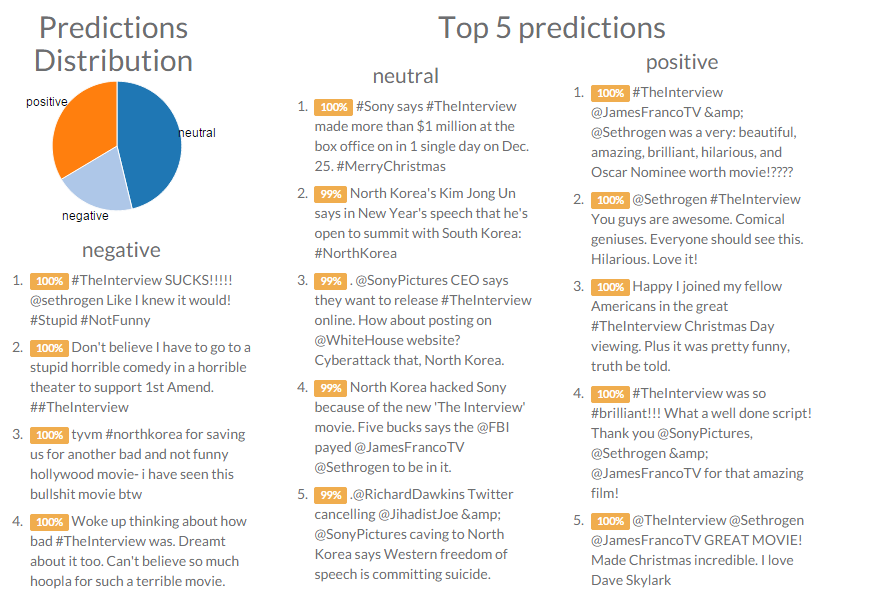
\includegraphics[width=\textwidth]{final_sentiment_theinterview}
  \caption[Sentiment - Sony Hack Concerning the Movie \enquote{The Interview}]{Sentiment - Sony Hack Concerning the Movie \enquote{The Interview}}
  \label{fig:sentiment-interview}
  \vspace{-1.3em}
\end{figure}

\subsection{Topic Modelling}
\label{subsec:topic-modelling}
Topic modeling is a statistical machine learning model for automatic discovery of abstract topics occurring in a collection of documents (content entities). Moreover, it allocates the analyzed documents to the discovered topics and clusters the most common words (terms). LDA is a common method of topic modeling introduced by Blei et al. \cite{Blei03lda}. The LDA method assumes that each document contains a mixture of topics where each word attributes to one of these topics \cite{Blei03lda}. The requirements for executing LDA for topic modelling are a collection of documents, a specified number of topics and specified number of iterations.

When analyzing detected trends on twitter we utilize LDA to find all topics related to hashtags. The documents needed for LDA are the collected tweets and the parameters topic count and iteration count are varied depending on the trend. Ramage et al. find in their research paper that the 140 characters of a tweet are sufficient as a document for LDA \cite{ramage2010lda}.

\begin{lstlisting}[caption={[Topic Model for the Sony hack concerning the movie \enquote{The Interview}] Topic Model for the Sony hack concerning the movie \enquote{The Interview}}, label={lst:topic-model-interview}, float=h]
  theinterview (1109) jamesfrancotv (782) sethrogen (573) movie (308) interview (204) funny (182) hilarious (148) °\DNumber°

  northkorea (253) sonyhack (140) korea (125) north (117) internet (75) sony (72) amp (57) °\DNumber°

  theinterview (695) sonypictures (264) sony (234) movie (147) korea (121) north (111) interview (100) °\DNumber°

  theinterview (223) aint (96) hate (76) cuz (58) jealous (52) anus (33) peanutbutter (26) °\DNumber°

  theinterview (537) christmas (132) day (89) theaters (67) freedom (66) theater (65) showing (57) °\DNumber°
\end{lstlisting}

Listing \ref{lst:topic-model-interview} shows the topics which were modelled by using LDA on all tweets related to the comedy \enquote{The Interview}. The results are based on nearly 5000 tweets, 5 topics and 1000 iterations. Every of those topics describes another aspect of this trend. The first topic probably covers recommendations for the movie itself while the second topic is about the hack of Sony Pictures. The third topic seems to be purely informational. The fourth topic references a hilarious scene from the movie which we do not want to spoiler in this paper. The last topic is about Sony's decision to stream the movie online and to show it in selected cinemas on christmas.

\subsection{Visualization}
\label{subsec:visualization}
To understand and interpret the results of this trend analysis, we used a variety of visualization techniques that help to get valuable insights about certain aspects.

\subsubsection{Time Series}
\label{subsubsec:vis-time-series}
The time series visualization is used to display the course of an event or a trend. It displays the dates in which the trend has been monitored on the horizontal axis against the count of tweets collected for that topic (based on our sampled twitter dataset) on the vertical axis. The analysis of the time series is particularly usable to detect new trends. Most trending topics will not show up in previous data at all, but as soon as they begin to spread on Twitter they will be clearly visible in the time series graph.

\begin{figure}[H]
  \centering
        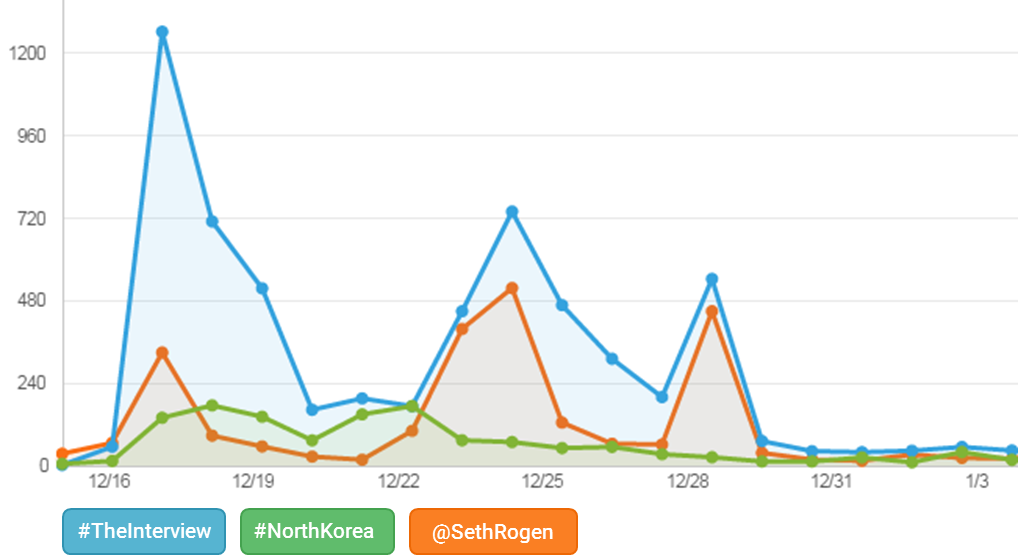
\includegraphics[width=\textwidth]{final_timeseries_theinterview}
  \caption[Time Series - Sony Hack Concerning the Movie \enquote{The Interview}]{Time Series - Sony Hack Concerning the Movie \enquote{The Interview}}
  \label{fig:time-series-interview}
  \vspace{-1.3em}
\end{figure}

Figure \ref{fig:time-series-interview} shows a time series visualization of the hashtags \textit{\#theinterview} and \textit{\#northkorea} and the user mention \textit{@SethRogen (main actor)} all belonging to the trend of the comedy movie \enquote{The Interview}. There is an observable peak for both hashtags and the user mention on 18\textsuperscript{th} of December when Sony announced that they will not screen the movie as a reaction to the hackers' threats. On 24\textsuperscript{th} of December Sony decided to make the movie available via online stream. This decision is visible as a peak in the time series visualization as well. The third and last peak in the visualization is based on a live tweeting event from main actor Seth Rogen who tweeted his comments and stories about the movie and the production \cite{deadline2014interview}.

\subsubsection{Word Cloud Visualization}
\label{subsubsec:vis-word-clouds}
The word cloud visualization highlights the most frequently occurring terms in the current twitter activity related to a trending topic. Thereby, the importance of a term is expressed using its font size. This visualization type is known as an effective summarizing technique and helps to detect the related topics to a trend.

The current implementation uses all tweets related to a trend and transforms them into a word cloud. Therefore all tweets are read from the database and then the frequency of each word in the text is counted using wordfreq.js\footnote{\url{http://timdream.org/wordfreq} \accessednote}. Finally, every unique word and the associated frequency is forwarded to wordcloud2.js\footnote{\url{http://timdream.org/wordcloud2.js} \accessednote}, a JavaScript visualization library, to render the corresponding word cloud.

\begin{figure}[H]
  \centering
        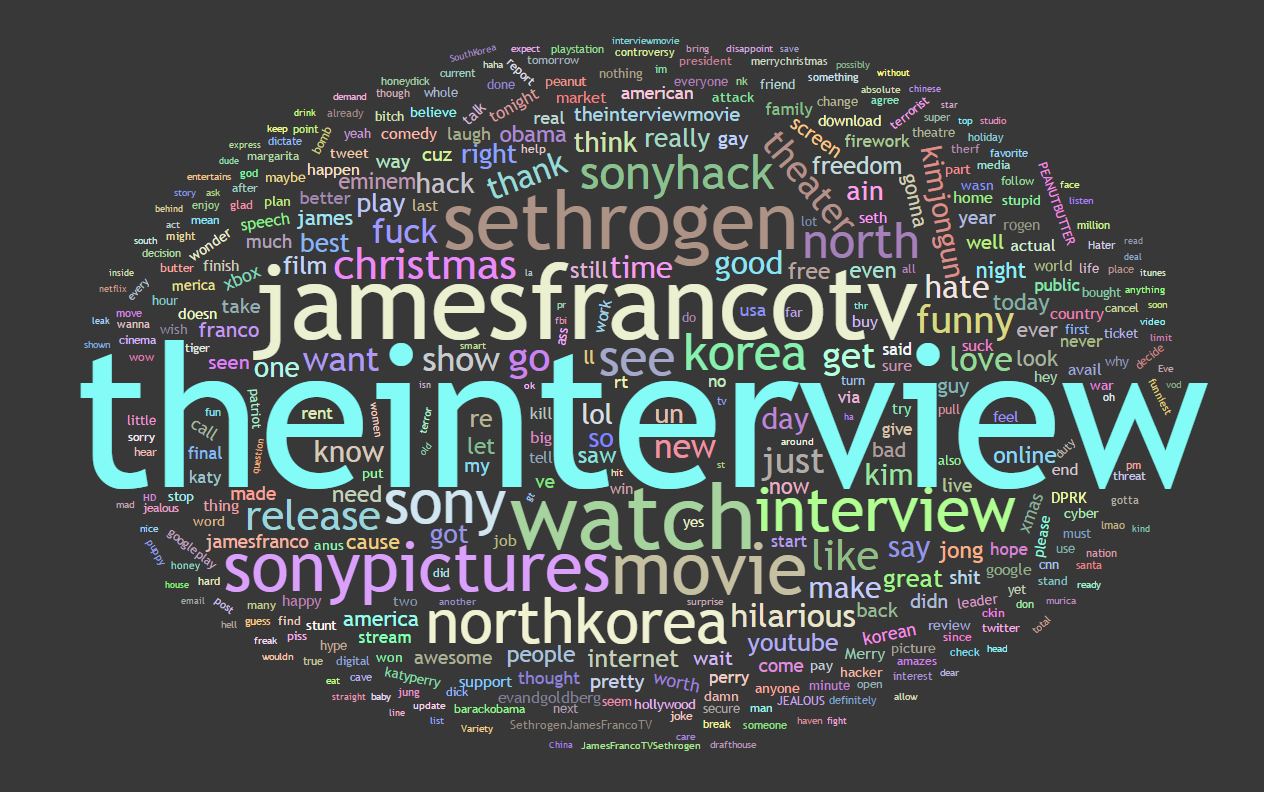
\includegraphics[width=\textwidth]{final_wordcloud_theinterview}
  \caption[Word Cloud - Sony Hack Concerning the Movie \enquote{The Interview}]{Word Cloud - Sony Hack Concerning the Movie \enquote{The Interview}}
  \label{fig:word-cloud-interview}
  \vspace{-1.3em}
\end{figure}

An example word cloud is visualized in figure \ref{fig:word-cloud-interview}. It shows the most common words for all tweets related to the comedy movie \enquote{The Interview}. The most frequent words were, of course, the movie title itself and the two main actors Seth Rogen and James Franco (his twitter username is \textit{@JamesFrancoTV}). Additionally, Sony Pictures and North Korea are mentioned quite often since they are strongly related to this trend. This example shows that a word cloud is a effective tool to quickly analyze the most frequent words of a trend.

\subsubsection{Geospatial Visualization}
\label{subsubsection:vis-geospatial}
Geospatial visualization helps to identify the location of current events and detect new events and trends that are likely to occur \cite{TwitterDataAnalytics2013}. Furthermore, it is used to gain insights into the prominent locations discussing a selected trend \cite[64-66]{TwitterDataAnalytics2013}. All visualizations are build with CartoDB\footnote{\url{http://cartodb.com} \accessednote}, a cloud-computing platform that provides mapping and visualization solutions for geolocated data.

\begin{figure}[H]
  \centering
        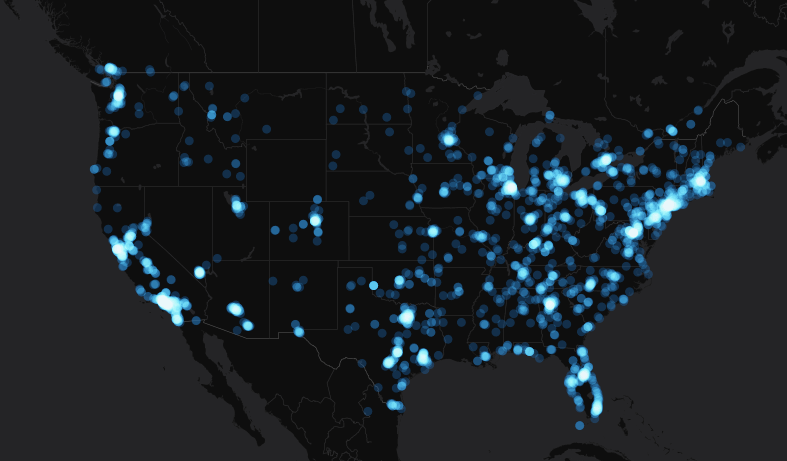
\includegraphics[width=\textwidth]{final_geospatial_map_theinterview}
  \caption[Geospatial analysis - Sony Hack Concerning the Movie \enquote{The Interview}]{Geospatial analysis - Sony Hack Concerning the Movie \enquote{The Interview}}
  \label{fig:map-interview}
  \vspace{-1.3em}
\end{figure}

A map enhanced with geospatial data is shown in figure \ref{fig:map-interview}. It displays tweets related to the comedy movie \enquote{The Interview}. The tweets are distributed equally over the whole United States of America. There are visible hotspots in the biggest cities New York, Los Angeles and San Francisco. The middle west has less tweets visible on the map which may be caused by a lower population in this area.

\section{Architecture}
\label{sec:architecture}

\begin{figure}[H]
  \centering
        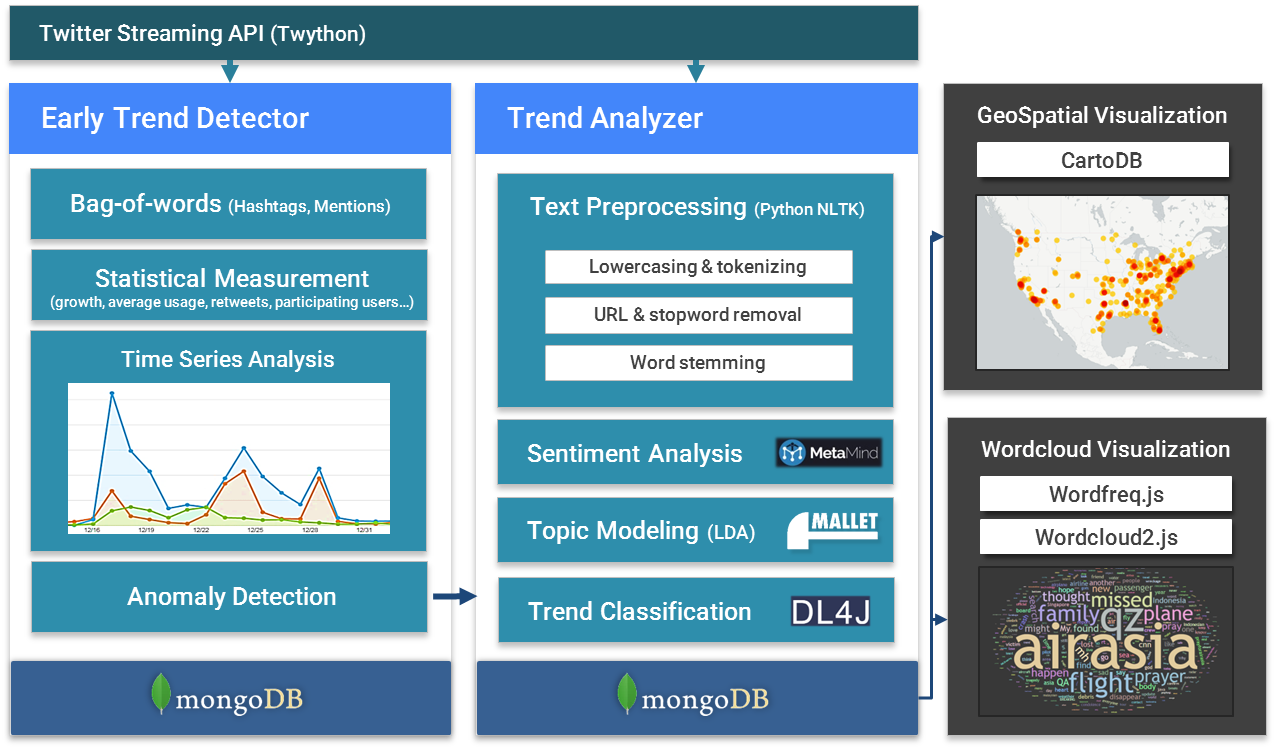
\includegraphics[width=\textwidth]{trend_detection_architecture}
  \caption[Trend Detection \& Analysis Dataflow Architecture]{Trend Detection \& Analysis Dataflow Architecture}
  \label{fig:twitter-trend-analysis-architecture}
\end{figure}


The implementation of our Twitter trend analysis tool, as presented in this paper, is separated into three main components: the Early Trend Detector, the Trend Analyzer and visualization tools. Thereby, the Early Trend Detector and the Trend Analyzer run in parallel on two different servers. Figure \ref{fig:twitter-trend-analysis-architecture} illustrates the architecture, implemented technologies and the data flow of our Twitter trend analysis tool.

The Early Trend Detector as well as the Trend Analyzer independently collect data from Twitter. Thereby, the collection of tweets from the Twitter Streaming API\footnote{Push service to collect public Tweets in real time.} is implemented with Python using Twython\footnote{\url{http://twython.readthedocs.org} \accessednote}. A Tweet contains a 140 character text message and various metadata such as the language, location, user information, number of retweets and favorites and more. The language used in Tweets is mostly informal and the correctness of grammar are often sacrificed to gain additional characters. Further, abbreviations and special characters (e.g. Emoticons) are also frequently employed \cite[67]{TwitterDataAnalytics2013}. We decided to lowercase the tweet text and hashtags to prevent ambiguity and complexity caused by case-sensitiveness. 

The main task of the \textbf{Early Trend Detector} is the early detection of upcoming Twitter trends. Therefore, this component streams data from Twitter filtered by English language and a bounding box on USA. These tweets are stored with an additional creation timestamp and all metadata from Twitter into MongoDB, a popular NoSQL database. In parallel, the Early Trend Detector also creates bag-of-words for hashtags and user mentions from incoming tweets and, additionally, calculates several statistics every twenty minutes such as average \& total occurrences, usage growth, participating users, retweet count and more. Based on these statistics, an anomaly detection process will be started every two hours to identify a list of about 10 unique hashtags and mentions with the highest trend potential. In the next step, one (or more) of those potential trends are selected and a list of correlated hashtags \& mentions is generated by querying and counting other hashtags \& mentions used in combination with the selected one. Finally, this list of hashtags and mentions related to a potential trend is forwarded to the Trend Analyzer component.

The \textbf{Trend Analyzer} aims to further monitor, observe and analyze the potential trend for additional insights. Therefore, this component streams data from Twitter filtered by English language and the list of hashtags and mentions related to the potential trend. To simplify the analysis task, each tweet is preprocessed using common NLP text preparation techniques. In the first step, the text of a tweet is lower-cased and special characters, URLs as well as English stop words get removed. The Tweet text is further simplified by using tokenizing and text stemming techniques. In the next step, the preprocessed Tweet text alongside with the original tweet text, creation timestamp and all metadata is stored in a separate MongoDB database. After the preprocessing, the sentiment (positive, neutral or negative) of every tweet is determined by using the sentiment classifier from MetaMind\footnote{\url{https://www.metamind.io} \accessednote}. Moreover, we utilize the topic modeling algorithm LDA from Mallet\footnote{\url{http://mallet.cs.umass.edu} \accessednote} to discover topics (word correlations) from the collected dataset of tweets related to the selected trend. 

To further analyze, understand and interpret our dataset for detected trends, we integrated a variety of visualization techniques that helps to get valuable insights about certain aspects (described in section \ref{subsec:visualization}). 